%% abtex2-modelo-artigo.tex, v<VERSION> laurocesar
%% Copyright 2012-<COPYRIGHT_YEAR> by abnTeX2 group at http://www.abntex.net.br/ 
%%
%% This work may be distributed and/or modified under the
%% conditions of the LaTeX Project Public License, either version 1.3
%% of this license or (at your option) any later version.
%% The latest version of this license is in
%%   http://www.latex-project.org/lppl.txt
%% and version 1.3 or later is part of all distributions of LaTeX
%% version 2005/12/01 or later.
%%
%% This work has the LPPL maintenance status `maintained'.
%% 
%% The Current Maintainer of this work is the abnTeX2 team, led
%% by Lauro César Araujo. Further information are available on 
%% http://www.abntex.net.br/
%%
%% This work consists of the files abntex2-modelo-artigo.tex and
%% abntex2-modelo-references.bib
%%

% ------------------------------------------------------------------------
% ------------------------------------------------------------------------
% abnTeX2: Modelo de Artigo Acadêmico em conformidade com
% ABNT NBR 6022:2003: Informação e documentação - Artigo em publicação 
% periódica científica impressa - Apresentação
% ------------------------------------------------------------------------
% ------------------------------------------------------------------------

\documentclass[
% -- opções da classe memoir --
article,			% indica que é um artigo acadêmico
11pt,				% tamanho da fonte
oneside,			% para impressão apenas no recto. Oposto a twoside
a4paper,			% tamanho do papel. 
% -- opções da classe abntex2 --
%chapter=TITLE,		% títulos de capítulos convertidos em letras maiúsculas
%section=TITLE,		% títulos de seções convertidos em letras maiúsculas
%subsection=TITLE,	% títulos de subseções convertidos em letras maiúsculas
%subsubsection=TITLE % títulos de subsubseções convertidos em letras maiúsculas
% -- opções do pacote babel --
english,			% idioma adicional para hifenização
brazil,				% o último idioma é o principal do documento
sumario=tradicional
]{article}


% ---
% PACOTES
% ---

% ---
% Pacotes fundamentais 
% ---
\usepackage[utf8]{inputenc}
\usepackage{graphicx}
\usepackage[export]{adjustbox}
\usepackage{float}
\usepackage[brazil]{babel}
\usepackage{indentfirst}
\usepackage[section]{placeins}
\usepackage{authblk}
\usepackage{lmodern}			% Usa a fonte Latin Modern
%\usepackage[T1]{fontenc}		% Selecao de codigos de fonte.
%\usepackage[utf8]{inputenc}		% Codificacao do documento (conversão automática dos acentos)
%\usepackage{indentfirst}		% Indenta o primeiro parágrafo de cada seção.
%\usepackage{nomencl} 			% Lista de simbolos
%\usepackage{color}				% Controle das cores
%\usepackage{graphicx}			% Inclusão de gráficos
%\usepackage{microtype} 			% para melhorias de justificação
% ---

% ---
% Pacotes adicionais, usados apenas no âmbito do Modelo Canônico do abnteX2
% ---
%\usepackage{lipsum}				% para geração de dummy text
% ---

\title{\textbf{Problema do caixeiro viajante utilizando Algoritimos Genéticos}}
\author{Diego Pontes Pasquini; Gabriela Araújo Coelho; Hugo Gustavo Valin Oliveira da Cunha; Jessiane Gomes Andrade; Tatiane Fernanda de Souza Silva}
\date{Dezembro de 2017}

% ----
% Início do documento
% ----
\begin{document}
	
	% página de titulo
	\maketitle
	
	\begin{center}
		\small
		Disciplina: Inteligência Computacional \\
		\small
		Professora: Dra. Rita Maria da Silva Julia
	\end{center}
	
	% resumo em português
	\begin{abstract}
		Neste trabalho foi implementado um programa utilizando Algoritimos Genéticos(AGs) com o objetivo de resolver o problema do caixeiro viajante. O projeto foi desenvolvido em linguagem Java, visando sua portabilidade.  	
		\vspace{20px}
		
		\noindent
		\textbf{Palavras-chave}: Algoritimos Genéticos. Inteligência Computacional. Caixeiro viajante.
	\end{abstract}
	

	\section{Introdução}
	\addcontentsline{toc}{section}{Introdução}

	A pesquisa sobre a área de Computação Evolutiva(CE) tem se expandido rapidamente, principalmente para resolver problemas de otimizaçãocombinatória NP-difícil.
	
	Os Algoritmos Evolutivos(AEs) são métodos de busca estocásticos que imitam a evolução biológica natural. Eles são compostos por uma sequência de passos até a solução, sendo estes passos os mesmos para uma ampla gama de problemas, fornecendo robustez e flexibilidade.
	
	Existem vantagens para utilizarmos esses algoritimos como o desenvolvimento de algoritmos capazes de encontrar soluções adequadas para problemas complexos, ainda não resolvidos por outras técnicas computacionais, a simplicidade dos métodos utilizando princípios básicos de Teoria da Evolução e Genética que podem ser modelados por poucas e simples linhas de código e também a adaptação relativamente fácil para problemas das mais diversas áreas.
	
	\vspace{10px}

	Os principais Algoritmos Evolutivos são:
	\begin{enumerate}
		\item Algoritmos Genéticos (AG);
		\item Estratégias Evolutivas (EE);
		\item Programação Evolutiva (PE);
		\item Programação Genética (PG); 
		\item Genetic Programming (GP);
		\item Sistemas Classificadores (SC);
	\end{enumerate}

	\subsection{Descrição do Problema Caixeiro Viajante}

	O Problema do Caixeiro Viajante (PCV) é um problema combinatório fundamentalmente matemático que tem perdurado por longo tempo. Não se sabe ao certo um documento que comprove sua autoria, muito menos a origem do nome. Em meados de 1800, problemas relacionados ao PCV começaram a ser desenvolvidos, mas somente em 1950 ficou conhecido globalmente em sua forma geral. \cite{APPLEGATE}.

	O PCV é um problema que tenta determinar a menor rota para percorrer uma série de cidades (visitando uma única vez cada uma delas), retornando à cidade de origem. Ele é um problema de otimização NP-difícil inspirado na necessidade dos vendedores em realizar entregas em diversos locais (as cidades) percorrendo o menor caminho possível, reduzindo o tempo necessário para a viagem e os possíveis custos com transporte e combustível.

	\begin{figure}[H]
		\centering
		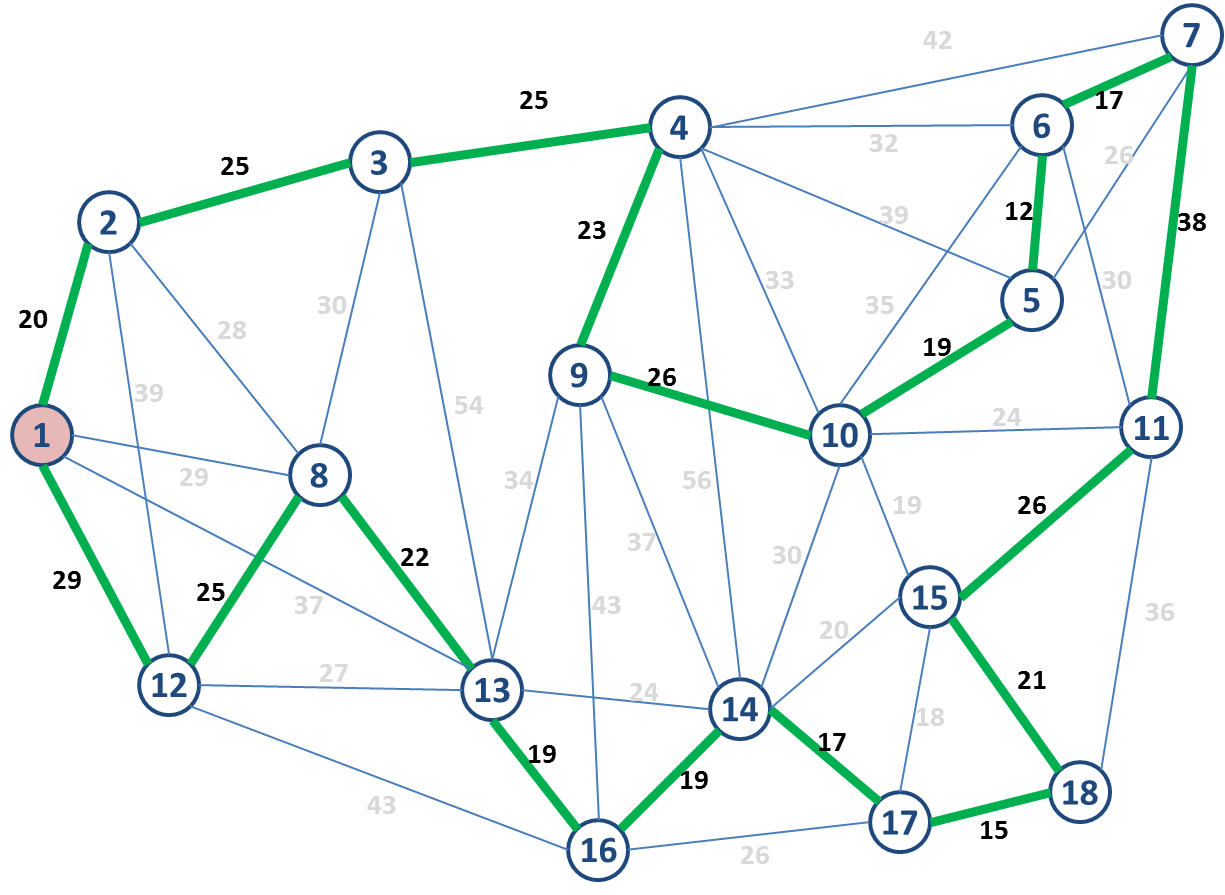
\includegraphics[width=0.7\textwidth]{Figuras/grafo-caixeiro-viajante.png}
		\caption{Exemplo de solução para um PVC.}
	\end{figure}

	Os algoritmos heurísticos constituem uma alternativa computacionalmente viável encontrada pelos pesquisadores para resolver o PCV. A limitação desta alternativa é a qualidade da solução obtida, que não necessariamente é a ótima. Dentre os métodos heurísticos que encontram soluções de forma eficiente estão os Algoritmos Genéticos(AGs).
	
	Os AGs são métodos de busca e otimização inspirados na biologia evolucionária da população de seres vivos \cite{DARWIN}\cite{HOLLAND} \cite{GOLDBERG}. Como uma técnica de otimização e busca, os algoritmos genéticos apresentam uma função objetivo (também chamado aptidão ou fitness), utilizada para avaliar cada uma de uma soluções obtidas, uma vez que o método gera um conjunto de soluções, e não apenas uma.
	
	\subsection{Aplicações} 
	
	Existem várias aplicações para o problema do caixeiro viajante. \cite{REINELT} Um exemplo é o processo de perfuração de placas de circuitos impressos em sua confecção. Uma placa de circuito impresso pode conter centenas ou milhares de furos para soldagem de componentes eletrônicos. Como os furos podem ser de tamanhos diferentes, é necessária a troca da ferramenta. Essa troca de ferramenta é um processo lento. Para que a ferramenta não seja trocada várias vezes, é necessária uma otimização perfurando primeiro todos os furos de mesmo diâmetro. Assim, esse processo pode ser visto como um problema do caixeiro viajante. Percorrendo-se o melhor caminho possível, economiza-se tempo, aumentando a produtividade do processo \cite{FREEDO}.
	
	Uma segunda aplicação é a que ocorre na análise de estruturas de cristais na cristalografia por raios-x. A cristalografia analisa a disposição dos átomos em sólidos. Para isso um difratômetro obtêm informações da estrutura de um material cristalino medindo a intensidade dos raios-x refletidos do material, saindo de várias posições. Em alguns experimentos, o difratômetro deve realizar até 30.000 deslocamentos para fazer as medidas. Isso significa que pode haver um percurso com até 30.000 pontos de medida. Para minimizar o tempo gasto na mensuração, deve-se escolher um percurso mínimo entre os pontos de medida, o qual pode ser modelado através do problema do caixeiro viajante \cite{FREEDO}.
	
	\section{Metodologia}
	
	Para o PCV, cada cromossomo codifica uma solução, isto é, a rota que possui a menor distância. A função de
	adaptação(fitness), que avalia cada cromossomo, está relacionada com o tamanho da rota, no qual depende da ordem em que as cidades aparecem na mesma.
	
	\begin{figure}[H]
		\centering
		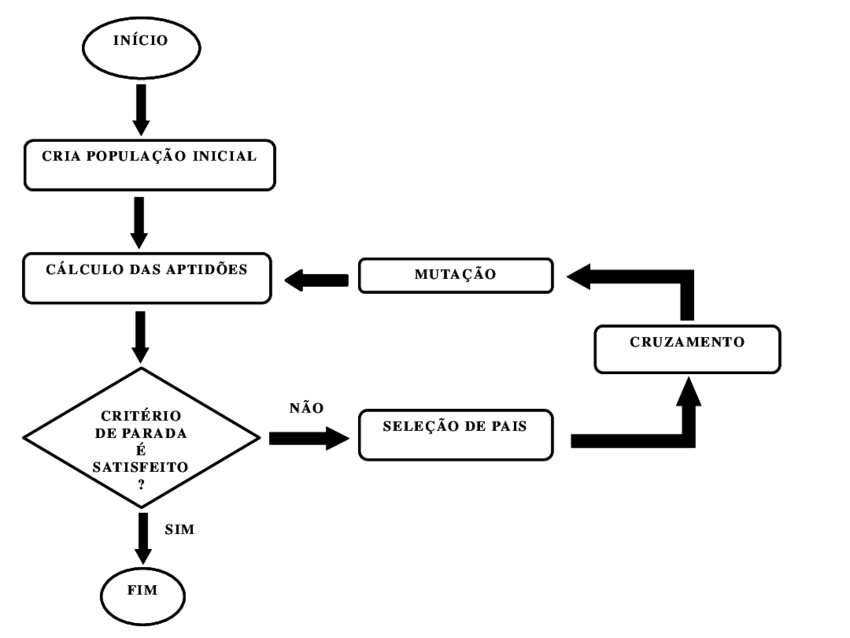
\includegraphics[width=1\textwidth]{Figuras/funcionamento-ag.png}
		\caption{Esquema geral de funcionamento do AG.}
	\end{figure}

	Foi utilizado uma matriz 42x42 para montar o grafo das cidades com as distâncias entre cada uma delas. 
	A representação de um cromossomo, para esta aplicação, é um vetor de tamanho 42 com a ordem a das cidades que irão ser percorridas. 
	
	Estrutura de um cromossomo: [d0,d1,d2,...,d41], onde d é a distância entre a cidade i e a cidade i-1.
	
	A aptidão(\textit{fitness}) é o cálculo da a distância total que é percorrida, sendo o objetivo é encontrar a menor distância.
	
	O método utilizado para fazer a seleção dos pais foi o método da roleta. Em seguida, a partir dos pais selecionados para a reprodução, é feito um \textit{Crossover} OX para gerar os filhos. Esses filhos sofrem mutação por um algoritimo de mutação pode inversão e ocorre a reincerção dos mesmo na população calculando a aptidão de cada um.
	
	
	\section{Configuração do AG}
	
	O programa implementado possui um arquivo de configurações onde fica bem mais simples mudar os valores dos elementos principais de um AG.
	Esse arquivo possui uma variável para guardar o número de gerações que o programa irá rodar, uma variável que irá guardar a quantidade de indivíduos que serão gerados na população inicial, a porcentagem de mutação que será sofrida pelos filhos gerados, a quantidade de vértices do grafo, e por último, a distância máxima percorrida. 
	

	\section{Resultados}
	
	Nos primeiros resultados podemos utilizamos a mutação que troca dois genes, ecolhidos aleatoriamente, de posição.

	\begin{figure}[H]
		\centering
		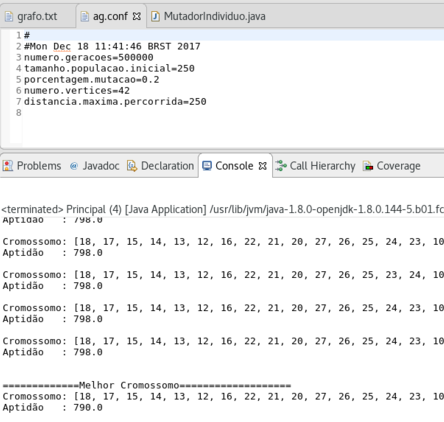
\includegraphics[width=1\textwidth]{Figuras/resultado-2genes.png}
		\caption{Resultado da mudança de aptidão através das gerações utilizando a mutação invertendo 2 genes.}
	\end{figure}
	
	\begin{figure}[H]
		\centering
		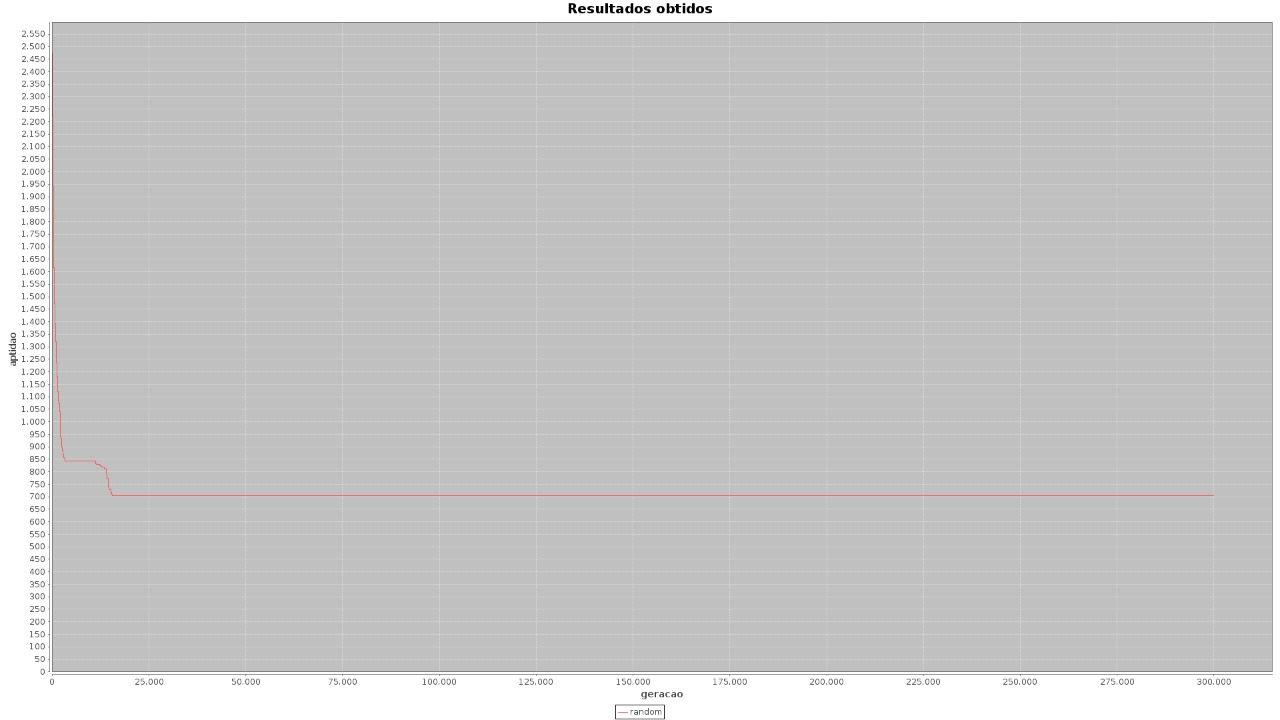
\includegraphics[width=1\textwidth]{Figuras/resultado1.jpeg}
		\caption{Evolução do AG através das gerações}
	\end{figure}

	Neste resultado podemos utilizamos a mutação que inverter uma sequência de genes, onde o ponto inicial e o ponto final da sequência são ecolhidos aleatoriamente.

	\begin{figure}[H]
		\centering
		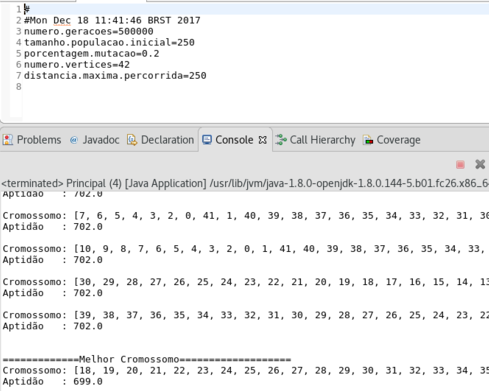
\includegraphics[width=1\textwidth]{Figuras/resultado-inversao.png}
		\caption{Resultado da mudança de aptidão através das gerações utilizando a mutação por inversão.}
	\end{figure}

	
	\section{Conclusão}
	
	Com esse trabalho podemos concluir que a escolha de bons métodos heurísticos para os problemas complexos fazem toda a diferença nos resultados.E, neste caso, comparando a mutação invertendo apenas dois genes do cromossomo com a mutação que inverte uma parte do cromossomo, podemos observar que no segundo caso chegmos em um resultado bem melhor.

	\begin{thebibliography}{4}
		\bibliographystyle{apa}
		
		\bibitem{APPLEGATE}
		David L. Applegate, Robert E. Bixby, Vasek Chvátal and William J. Cook
		\emph{The Traveling Salesman Problem. A Computational Study},
		Princeton University Press,
		2006
		
		\bibitem{DARWIN}
		Darwin, Charles
		\emph{The Traveling Salesman Problem. On the Origin of Species by Means of Natural Selection},
		London
		1859
		
		\bibitem{HOLLAND}
		Holland, John H.
		\emph{Adaptation in Natural and Artificial Systems},
		Ann Arbor, MI
		1975
		
		\bibitem{GOLDBERG}
		Goldberg, David E.
		\emph{Genetic Algorithms in Search, Optimization, and Machine Learning},
		1989
		
		\bibitem{REINELT}
		Reinelt, G.
		\emph{The Traveling Salesman: Computational Solutions for TSP Applications},
		Lecture Notes in Computer Science, 840, Springer-Verlag,
		1994
		
		\bibitem{FREEDO}
		Freddo, Ademir Roberto and Brito, Robison Cris.
		\emph{Implementação da Metaheurística GRASP para o Problema
			do Caixeiro Viajante Simétrico}.
		Disponível em: http://www.inf.ufpr.br/aurora/disciplinas/topicosia2/
		downloads/trabalhos/GraspTSP.pdf.
		Acesso em: 19/12/2017
			
	\end{thebibliography}
	
\end{document}